% Created by tikzDevice version 0.6.2-92-0ad2792 on 2013-04-07 18:08:56
% !TEX encoding = UTF-8 Unicode
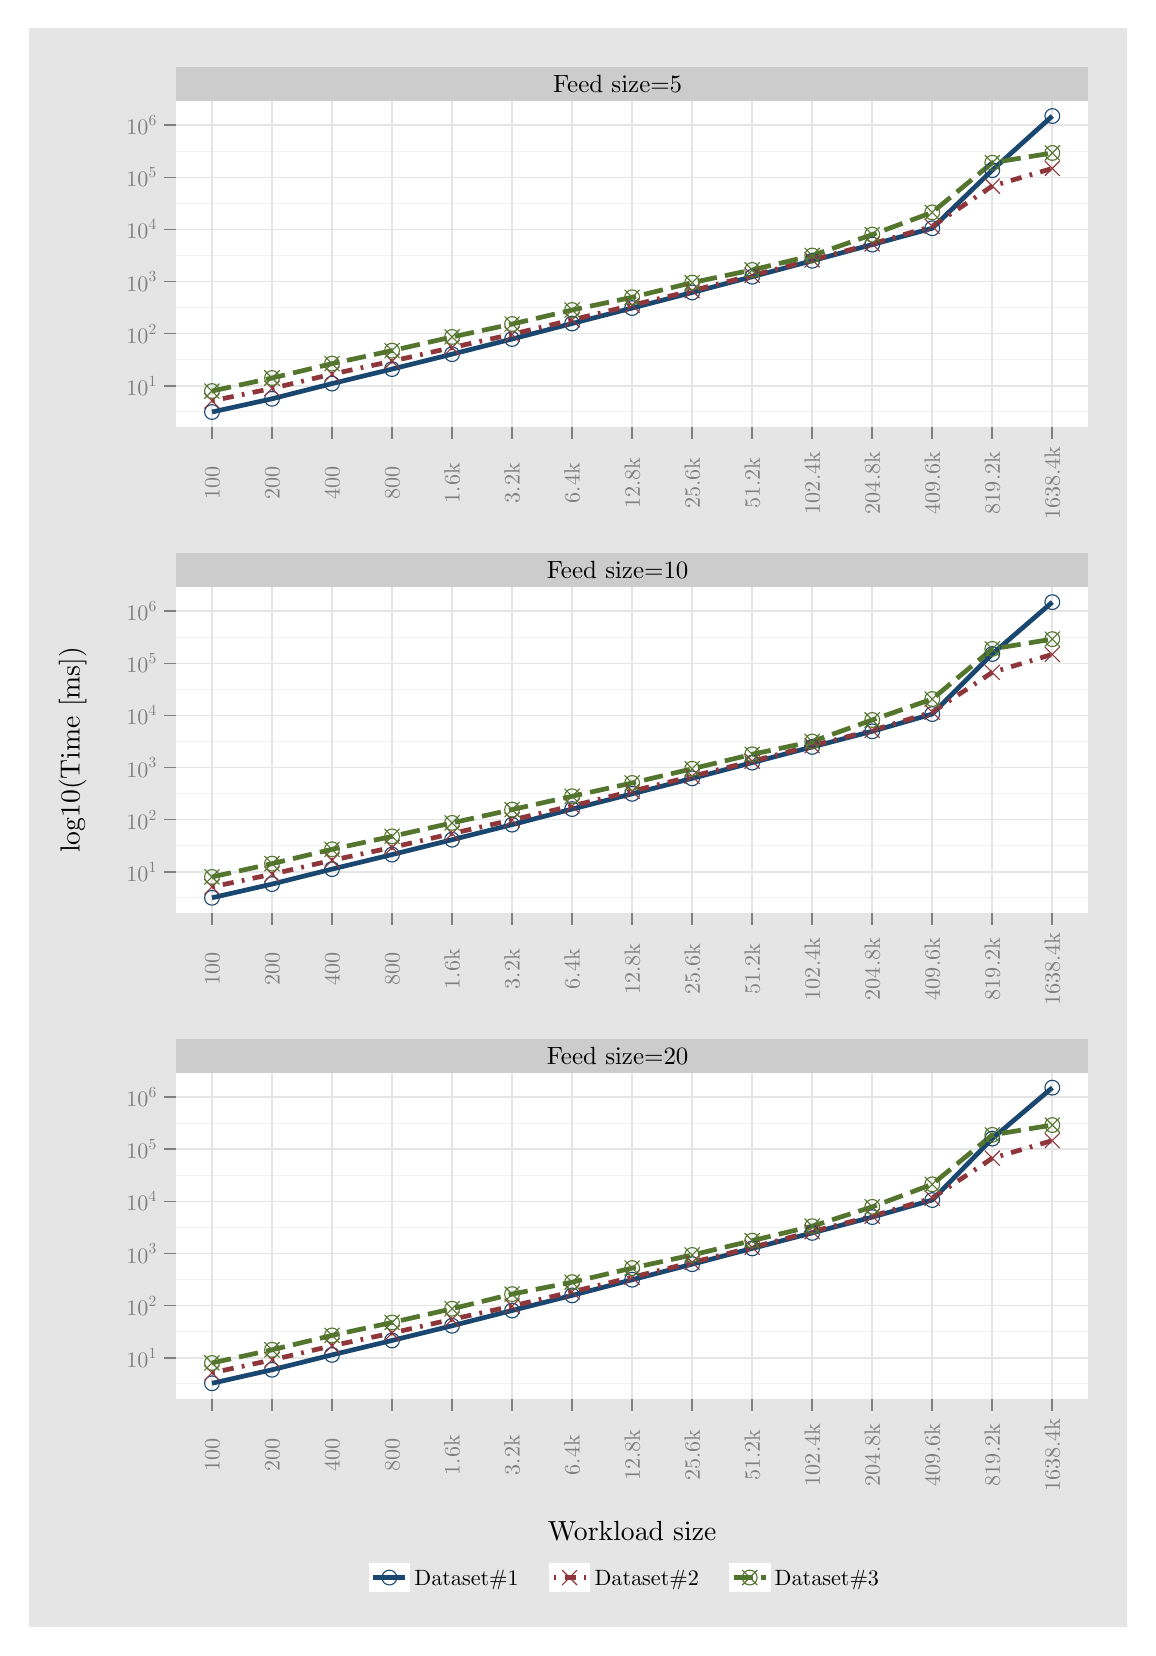
\begin{tikzpicture}[x=1pt,y=1pt]
\definecolor[named]{fillColor}{rgb}{1.00,1.00,1.00}
\path[use as bounding box,fill=fillColor,fill opacity=0.00] (0,0) rectangle (397.48,578.16);
\begin{scope}
\path[clip] (  0.00,  0.00) rectangle (397.48,578.16);
\definecolor[named]{drawColor}{rgb}{1.00,1.00,1.00}
\definecolor[named]{fillColor}{rgb}{0.90,0.90,0.90}

\path[draw=drawColor,line width= 0.6pt,line join=round,line cap=round,fill=fillColor] (  0.00,  0.00) rectangle (397.48,578.16);
\end{scope}
\begin{scope}
\path[clip] ( 53.58,433.92) rectangle (383.26,551.71);
\definecolor[named]{fillColor}{rgb}{1.00,1.00,1.00}

\path[fill=fillColor] ( 53.58,433.92) rectangle (383.26,551.71);
\definecolor[named]{drawColor}{rgb}{0.95,0.95,0.95}

\path[draw=drawColor,line width= 0.3pt,line join=round] ( 53.58,439.35) --
	(383.26,439.35);

\path[draw=drawColor,line width= 0.3pt,line join=round] ( 53.58,458.18) --
	(383.26,458.18);

\path[draw=drawColor,line width= 0.3pt,line join=round] ( 53.58,477.01) --
	(383.26,477.01);

\path[draw=drawColor,line width= 0.3pt,line join=round] ( 53.58,495.83) --
	(383.26,495.83);

\path[draw=drawColor,line width= 0.3pt,line join=round] ( 53.58,514.66) --
	(383.26,514.66);

\path[draw=drawColor,line width= 0.3pt,line join=round] ( 53.58,533.48) --
	(383.26,533.48);
\definecolor[named]{drawColor}{rgb}{0.90,0.90,0.90}

\path[draw=drawColor,line width= 0.6pt,line join=round] ( 53.58,448.77) --
	(383.26,448.77);

\path[draw=drawColor,line width= 0.6pt,line join=round] ( 53.58,467.59) --
	(383.26,467.59);

\path[draw=drawColor,line width= 0.6pt,line join=round] ( 53.58,486.42) --
	(383.26,486.42);

\path[draw=drawColor,line width= 0.6pt,line join=round] ( 53.58,505.25) --
	(383.26,505.25);

\path[draw=drawColor,line width= 0.6pt,line join=round] ( 53.58,524.07) --
	(383.26,524.07);

\path[draw=drawColor,line width= 0.6pt,line join=round] ( 53.58,542.90) --
	(383.26,542.90);

\path[draw=drawColor,line width= 0.6pt,line join=round] ( 66.60,433.92) --
	( 66.60,551.71);

\path[draw=drawColor,line width= 0.6pt,line join=round] ( 88.29,433.92) --
	( 88.29,551.71);

\path[draw=drawColor,line width= 0.6pt,line join=round] (109.97,433.92) --
	(109.97,551.71);

\path[draw=drawColor,line width= 0.6pt,line join=round] (131.66,433.92) --
	(131.66,551.71);

\path[draw=drawColor,line width= 0.6pt,line join=round] (153.35,433.92) --
	(153.35,551.71);

\path[draw=drawColor,line width= 0.6pt,line join=round] (175.04,433.92) --
	(175.04,551.71);

\path[draw=drawColor,line width= 0.6pt,line join=round] (196.73,433.92) --
	(196.73,551.71);

\path[draw=drawColor,line width= 0.6pt,line join=round] (218.42,433.92) --
	(218.42,551.71);

\path[draw=drawColor,line width= 0.6pt,line join=round] (240.11,433.92) --
	(240.11,551.71);

\path[draw=drawColor,line width= 0.6pt,line join=round] (261.80,433.92) --
	(261.80,551.71);

\path[draw=drawColor,line width= 0.6pt,line join=round] (283.49,433.92) --
	(283.49,551.71);

\path[draw=drawColor,line width= 0.6pt,line join=round] (305.18,433.92) --
	(305.18,551.71);

\path[draw=drawColor,line width= 0.6pt,line join=round] (326.87,433.92) --
	(326.87,551.71);

\path[draw=drawColor,line width= 0.6pt,line join=round] (348.56,433.92) --
	(348.56,551.71);

\path[draw=drawColor,line width= 0.6pt,line join=round] (370.25,433.92) --
	(370.25,551.71);
\definecolor[named]{drawColor}{rgb}{0.10,0.28,0.44}

\path[draw=drawColor,line width= 1.7pt,line join=round] ( 66.60,439.27) --
	( 88.29,444.05) --
	(109.97,449.54) --
	(131.66,454.79) --
	(153.35,460.17) --
	(175.04,465.65) --
	(196.73,471.26) --
	(218.42,476.84) --
	(240.11,482.47) --
	(261.80,488.16) --
	(283.49,493.93) --
	(305.18,499.77) --
	(326.87,505.67) --
	(348.56,526.67) --
	(370.25,546.23);
\definecolor[named]{drawColor}{rgb}{0.56,0.21,0.23}

\path[draw=drawColor,line width= 1.7pt,dash pattern=on 1pt off 3pt on 4pt off 3pt ,line join=round] ( 66.60,443.31) --
	( 88.29,447.79) --
	(109.97,452.96) --
	(131.66,457.64) --
	(153.35,462.56) --
	(175.04,467.38) --
	(196.73,472.56) --
	(218.42,477.88) --
	(240.11,483.11) --
	(261.80,488.66) --
	(283.49,494.26) --
	(305.18,500.06) --
	(326.87,506.38) --
	(348.56,520.93) --
	(370.25,527.29);
\definecolor[named]{drawColor}{rgb}{0.33,0.46,0.18}

\path[draw=drawColor,line width= 1.7pt,dash pattern=on 7pt off 3pt ,line join=round] ( 66.60,446.85) --
	( 88.29,451.56) --
	(109.97,456.76) --
	(131.66,461.45) --
	(153.35,466.39) --
	(175.04,471.06) --
	(196.73,476.13) --
	(218.42,480.73) --
	(240.11,486.03) --
	(261.80,490.61) --
	(283.49,495.82) --
	(305.18,503.38) --
	(326.87,511.41) --
	(348.56,529.36) --
	(370.25,532.88);
\definecolor[named]{drawColor}{rgb}{0.10,0.28,0.44}

\path[draw=drawColor,line width= 0.4pt,line join=round,line cap=round] ( 66.60,439.27) circle (  2.67);

\path[draw=drawColor,line width= 0.4pt,line join=round,line cap=round] ( 88.29,444.05) circle (  2.67);

\path[draw=drawColor,line width= 0.4pt,line join=round,line cap=round] (109.97,449.54) circle (  2.67);

\path[draw=drawColor,line width= 0.4pt,line join=round,line cap=round] (131.66,454.79) circle (  2.67);

\path[draw=drawColor,line width= 0.4pt,line join=round,line cap=round] (153.35,460.17) circle (  2.67);

\path[draw=drawColor,line width= 0.4pt,line join=round,line cap=round] (175.04,465.65) circle (  2.67);

\path[draw=drawColor,line width= 0.4pt,line join=round,line cap=round] (196.73,471.26) circle (  2.67);

\path[draw=drawColor,line width= 0.4pt,line join=round,line cap=round] (218.42,476.84) circle (  2.67);

\path[draw=drawColor,line width= 0.4pt,line join=round,line cap=round] (240.11,482.47) circle (  2.67);

\path[draw=drawColor,line width= 0.4pt,line join=round,line cap=round] (261.80,488.16) circle (  2.67);

\path[draw=drawColor,line width= 0.4pt,line join=round,line cap=round] (283.49,493.93) circle (  2.67);

\path[draw=drawColor,line width= 0.4pt,line join=round,line cap=round] (305.18,499.77) circle (  2.67);

\path[draw=drawColor,line width= 0.4pt,line join=round,line cap=round] (326.87,505.67) circle (  2.67);

\path[draw=drawColor,line width= 0.4pt,line join=round,line cap=round] (348.56,526.67) circle (  2.67);

\path[draw=drawColor,line width= 0.4pt,line join=round,line cap=round] (370.25,546.23) circle (  2.67);
\definecolor[named]{drawColor}{rgb}{0.56,0.21,0.23}

\path[draw=drawColor,line width= 0.4pt,line join=round,line cap=round,fill=fillColor] ( 63.93,440.64) -- ( 69.26,445.98);

\path[draw=drawColor,line width= 0.4pt,line join=round,line cap=round,fill=fillColor] ( 63.93,445.98) -- ( 69.26,440.64);

\path[draw=drawColor,line width= 0.4pt,line join=round,line cap=round,fill=fillColor] ( 85.62,445.13) -- ( 90.95,450.46);

\path[draw=drawColor,line width= 0.4pt,line join=round,line cap=round,fill=fillColor] ( 85.62,450.46) -- ( 90.95,445.13);

\path[draw=drawColor,line width= 0.4pt,line join=round,line cap=round,fill=fillColor] (107.31,450.29) -- (112.64,455.63);

\path[draw=drawColor,line width= 0.4pt,line join=round,line cap=round,fill=fillColor] (107.31,455.63) -- (112.64,450.29);

\path[draw=drawColor,line width= 0.4pt,line join=round,line cap=round,fill=fillColor] (129.00,454.97) -- (134.33,460.31);

\path[draw=drawColor,line width= 0.4pt,line join=round,line cap=round,fill=fillColor] (129.00,460.31) -- (134.33,454.97);

\path[draw=drawColor,line width= 0.4pt,line join=round,line cap=round,fill=fillColor] (150.69,459.89) -- (156.02,465.23);

\path[draw=drawColor,line width= 0.4pt,line join=round,line cap=round,fill=fillColor] (150.69,465.23) -- (156.02,459.89);

\path[draw=drawColor,line width= 0.4pt,line join=round,line cap=round,fill=fillColor] (172.37,464.71) -- (177.71,470.04);

\path[draw=drawColor,line width= 0.4pt,line join=round,line cap=round,fill=fillColor] (172.37,470.04) -- (177.71,464.71);

\path[draw=drawColor,line width= 0.4pt,line join=round,line cap=round,fill=fillColor] (194.06,469.90) -- (199.40,475.23);

\path[draw=drawColor,line width= 0.4pt,line join=round,line cap=round,fill=fillColor] (194.06,475.23) -- (199.40,469.90);

\path[draw=drawColor,line width= 0.4pt,line join=round,line cap=round,fill=fillColor] (215.75,475.21) -- (221.09,480.55);

\path[draw=drawColor,line width= 0.4pt,line join=round,line cap=round,fill=fillColor] (215.75,480.55) -- (221.09,475.21);

\path[draw=drawColor,line width= 0.4pt,line join=round,line cap=round,fill=fillColor] (237.44,480.44) -- (242.78,485.78);

\path[draw=drawColor,line width= 0.4pt,line join=round,line cap=round,fill=fillColor] (237.44,485.78) -- (242.78,480.44);

\path[draw=drawColor,line width= 0.4pt,line join=round,line cap=round,fill=fillColor] (259.13,485.99) -- (264.47,491.33);

\path[draw=drawColor,line width= 0.4pt,line join=round,line cap=round,fill=fillColor] (259.13,491.33) -- (264.47,485.99);

\path[draw=drawColor,line width= 0.4pt,line join=round,line cap=round,fill=fillColor] (280.82,491.59) -- (286.16,496.93);

\path[draw=drawColor,line width= 0.4pt,line join=round,line cap=round,fill=fillColor] (280.82,496.93) -- (286.16,491.59);

\path[draw=drawColor,line width= 0.4pt,line join=round,line cap=round,fill=fillColor] (302.51,497.40) -- (307.84,502.73);

\path[draw=drawColor,line width= 0.4pt,line join=round,line cap=round,fill=fillColor] (302.51,502.73) -- (307.84,497.40);

\path[draw=drawColor,line width= 0.4pt,line join=round,line cap=round,fill=fillColor] (324.20,503.71) -- (329.53,509.04);

\path[draw=drawColor,line width= 0.4pt,line join=round,line cap=round,fill=fillColor] (324.20,509.04) -- (329.53,503.71);

\path[draw=drawColor,line width= 0.4pt,line join=round,line cap=round,fill=fillColor] (345.89,518.26) -- (351.22,523.60);

\path[draw=drawColor,line width= 0.4pt,line join=round,line cap=round,fill=fillColor] (345.89,523.60) -- (351.22,518.26);

\path[draw=drawColor,line width= 0.4pt,line join=round,line cap=round,fill=fillColor] (367.58,524.63) -- (372.91,529.96);

\path[draw=drawColor,line width= 0.4pt,line join=round,line cap=round,fill=fillColor] (367.58,529.96) -- (372.91,524.63);
\definecolor[named]{drawColor}{rgb}{0.33,0.46,0.18}

\path[draw=drawColor,line width= 0.4pt,line join=round,line cap=round] ( 66.60,446.85) circle (  2.67);

\path[draw=drawColor,line width= 0.4pt,line join=round,line cap=round] ( 63.93,444.18) -- ( 69.26,449.52);

\path[draw=drawColor,line width= 0.4pt,line join=round,line cap=round] ( 63.93,449.52) -- ( 69.26,444.18);

\path[draw=drawColor,line width= 0.4pt,line join=round,line cap=round] ( 88.29,451.56) circle (  2.67);

\path[draw=drawColor,line width= 0.4pt,line join=round,line cap=round] ( 85.62,448.89) -- ( 90.95,454.23);

\path[draw=drawColor,line width= 0.4pt,line join=round,line cap=round] ( 85.62,454.23) -- ( 90.95,448.89);

\path[draw=drawColor,line width= 0.4pt,line join=round,line cap=round] (109.97,456.76) circle (  2.67);

\path[draw=drawColor,line width= 0.4pt,line join=round,line cap=round] (107.31,454.10) -- (112.64,459.43);

\path[draw=drawColor,line width= 0.4pt,line join=round,line cap=round] (107.31,459.43) -- (112.64,454.10);

\path[draw=drawColor,line width= 0.4pt,line join=round,line cap=round] (131.66,461.45) circle (  2.67);

\path[draw=drawColor,line width= 0.4pt,line join=round,line cap=round] (129.00,458.78) -- (134.33,464.12);

\path[draw=drawColor,line width= 0.4pt,line join=round,line cap=round] (129.00,464.12) -- (134.33,458.78);

\path[draw=drawColor,line width= 0.4pt,line join=round,line cap=round] (153.35,466.39) circle (  2.67);

\path[draw=drawColor,line width= 0.4pt,line join=round,line cap=round] (150.69,463.73) -- (156.02,469.06);

\path[draw=drawColor,line width= 0.4pt,line join=round,line cap=round] (150.69,469.06) -- (156.02,463.73);

\path[draw=drawColor,line width= 0.4pt,line join=round,line cap=round] (175.04,471.06) circle (  2.67);

\path[draw=drawColor,line width= 0.4pt,line join=round,line cap=round] (172.37,468.39) -- (177.71,473.73);

\path[draw=drawColor,line width= 0.4pt,line join=round,line cap=round] (172.37,473.73) -- (177.71,468.39);

\path[draw=drawColor,line width= 0.4pt,line join=round,line cap=round] (196.73,476.13) circle (  2.67);

\path[draw=drawColor,line width= 0.4pt,line join=round,line cap=round] (194.06,473.46) -- (199.40,478.80);

\path[draw=drawColor,line width= 0.4pt,line join=round,line cap=round] (194.06,478.80) -- (199.40,473.46);

\path[draw=drawColor,line width= 0.4pt,line join=round,line cap=round] (218.42,480.73) circle (  2.67);

\path[draw=drawColor,line width= 0.4pt,line join=round,line cap=round] (215.75,478.06) -- (221.09,483.40);

\path[draw=drawColor,line width= 0.4pt,line join=round,line cap=round] (215.75,483.40) -- (221.09,478.06);

\path[draw=drawColor,line width= 0.4pt,line join=round,line cap=round] (240.11,486.03) circle (  2.67);

\path[draw=drawColor,line width= 0.4pt,line join=round,line cap=round] (237.44,483.36) -- (242.78,488.69);

\path[draw=drawColor,line width= 0.4pt,line join=round,line cap=round] (237.44,488.69) -- (242.78,483.36);

\path[draw=drawColor,line width= 0.4pt,line join=round,line cap=round] (261.80,490.61) circle (  2.67);

\path[draw=drawColor,line width= 0.4pt,line join=round,line cap=round] (259.13,487.94) -- (264.47,493.28);

\path[draw=drawColor,line width= 0.4pt,line join=round,line cap=round] (259.13,493.28) -- (264.47,487.94);

\path[draw=drawColor,line width= 0.4pt,line join=round,line cap=round] (283.49,495.82) circle (  2.67);

\path[draw=drawColor,line width= 0.4pt,line join=round,line cap=round] (280.82,493.15) -- (286.16,498.49);

\path[draw=drawColor,line width= 0.4pt,line join=round,line cap=round] (280.82,498.49) -- (286.16,493.15);

\path[draw=drawColor,line width= 0.4pt,line join=round,line cap=round] (305.18,503.38) circle (  2.67);

\path[draw=drawColor,line width= 0.4pt,line join=round,line cap=round] (302.51,500.71) -- (307.84,506.05);

\path[draw=drawColor,line width= 0.4pt,line join=round,line cap=round] (302.51,506.05) -- (307.84,500.71);

\path[draw=drawColor,line width= 0.4pt,line join=round,line cap=round] (326.87,511.41) circle (  2.67);

\path[draw=drawColor,line width= 0.4pt,line join=round,line cap=round] (324.20,508.74) -- (329.53,514.07);

\path[draw=drawColor,line width= 0.4pt,line join=round,line cap=round] (324.20,514.07) -- (329.53,508.74);

\path[draw=drawColor,line width= 0.4pt,line join=round,line cap=round] (348.56,529.36) circle (  2.67);

\path[draw=drawColor,line width= 0.4pt,line join=round,line cap=round] (345.89,526.69) -- (351.22,532.02);

\path[draw=drawColor,line width= 0.4pt,line join=round,line cap=round] (345.89,532.02) -- (351.22,526.69);

\path[draw=drawColor,line width= 0.4pt,line join=round,line cap=round] (370.25,532.88) circle (  2.67);

\path[draw=drawColor,line width= 0.4pt,line join=round,line cap=round] (367.58,530.21) -- (372.91,535.54);

\path[draw=drawColor,line width= 0.4pt,line join=round,line cap=round] (367.58,535.54) -- (372.91,530.21);
\end{scope}
\begin{scope}
\path[clip] ( 53.58,258.30) rectangle (383.26,376.10);
\definecolor[named]{fillColor}{rgb}{1.00,1.00,1.00}

\path[fill=fillColor] ( 53.58,258.30) rectangle (383.26,376.10);
\definecolor[named]{drawColor}{rgb}{0.95,0.95,0.95}

\path[draw=drawColor,line width= 0.3pt,line join=round] ( 53.58,263.74) --
	(383.26,263.74);

\path[draw=drawColor,line width= 0.3pt,line join=round] ( 53.58,282.57) --
	(383.26,282.57);

\path[draw=drawColor,line width= 0.3pt,line join=round] ( 53.58,301.39) --
	(383.26,301.39);

\path[draw=drawColor,line width= 0.3pt,line join=round] ( 53.58,320.22) --
	(383.26,320.22);

\path[draw=drawColor,line width= 0.3pt,line join=round] ( 53.58,339.05) --
	(383.26,339.05);

\path[draw=drawColor,line width= 0.3pt,line join=round] ( 53.58,357.87) --
	(383.26,357.87);
\definecolor[named]{drawColor}{rgb}{0.90,0.90,0.90}

\path[draw=drawColor,line width= 0.6pt,line join=round] ( 53.58,273.15) --
	(383.26,273.15);

\path[draw=drawColor,line width= 0.6pt,line join=round] ( 53.58,291.98) --
	(383.26,291.98);

\path[draw=drawColor,line width= 0.6pt,line join=round] ( 53.58,310.81) --
	(383.26,310.81);

\path[draw=drawColor,line width= 0.6pt,line join=round] ( 53.58,329.63) --
	(383.26,329.63);

\path[draw=drawColor,line width= 0.6pt,line join=round] ( 53.58,348.46) --
	(383.26,348.46);

\path[draw=drawColor,line width= 0.6pt,line join=round] ( 53.58,367.28) --
	(383.26,367.28);

\path[draw=drawColor,line width= 0.6pt,line join=round] ( 66.60,258.30) --
	( 66.60,376.10);

\path[draw=drawColor,line width= 0.6pt,line join=round] ( 88.29,258.30) --
	( 88.29,376.10);

\path[draw=drawColor,line width= 0.6pt,line join=round] (109.97,258.30) --
	(109.97,376.10);

\path[draw=drawColor,line width= 0.6pt,line join=round] (131.66,258.30) --
	(131.66,376.10);

\path[draw=drawColor,line width= 0.6pt,line join=round] (153.35,258.30) --
	(153.35,376.10);

\path[draw=drawColor,line width= 0.6pt,line join=round] (175.04,258.30) --
	(175.04,376.10);

\path[draw=drawColor,line width= 0.6pt,line join=round] (196.73,258.30) --
	(196.73,376.10);

\path[draw=drawColor,line width= 0.6pt,line join=round] (218.42,258.30) --
	(218.42,376.10);

\path[draw=drawColor,line width= 0.6pt,line join=round] (240.11,258.30) --
	(240.11,376.10);

\path[draw=drawColor,line width= 0.6pt,line join=round] (261.80,258.30) --
	(261.80,376.10);

\path[draw=drawColor,line width= 0.6pt,line join=round] (283.49,258.30) --
	(283.49,376.10);

\path[draw=drawColor,line width= 0.6pt,line join=round] (305.18,258.30) --
	(305.18,376.10);

\path[draw=drawColor,line width= 0.6pt,line join=round] (326.87,258.30) --
	(326.87,376.10);

\path[draw=drawColor,line width= 0.6pt,line join=round] (348.56,258.30) --
	(348.56,376.10);

\path[draw=drawColor,line width= 0.6pt,line join=round] (370.25,258.30) --
	(370.25,376.10);
\definecolor[named]{drawColor}{rgb}{0.10,0.28,0.44}

\path[draw=drawColor,line width= 1.7pt,line join=round] ( 66.60,263.74) --
	( 88.29,268.69) --
	(109.97,274.10) --
	(131.66,279.35) --
	(153.35,284.72) --
	(175.04,290.17) --
	(196.73,295.80) --
	(218.42,301.30) --
	(240.11,306.89) --
	(261.80,312.58) --
	(283.49,318.26) --
	(305.18,323.90) --
	(326.87,330.13) --
	(348.56,351.83) --
	(370.25,370.57);
\definecolor[named]{drawColor}{rgb}{0.56,0.21,0.23}

\path[draw=drawColor,line width= 1.7pt,dash pattern=on 1pt off 3pt on 4pt off 3pt ,line join=round] ( 66.60,267.67) --
	( 88.29,272.26) --
	(109.97,277.29) --
	(131.66,281.93) --
	(153.35,286.96) --
	(175.04,291.88) --
	(196.73,296.94) --
	(218.42,302.27) --
	(240.11,307.65) --
	(261.80,313.09) --
	(283.49,318.73) --
	(305.18,324.25) --
	(326.87,330.83) --
	(348.56,345.21) --
	(370.25,351.69);
\definecolor[named]{drawColor}{rgb}{0.33,0.46,0.18}

\path[draw=drawColor,line width= 1.7pt,dash pattern=on 7pt off 3pt ,line join=round] ( 66.60,271.27) --
	( 88.29,276.08) --
	(109.97,281.26) --
	(131.66,285.93) --
	(153.35,290.80) --
	(175.04,295.61) --
	(196.73,300.44) --
	(218.42,305.23) --
	(240.11,310.35) --
	(261.80,315.58) --
	(283.49,320.21) --
	(305.18,327.99) --
	(326.87,335.56) --
	(348.56,353.67) --
	(370.25,357.20);
\definecolor[named]{drawColor}{rgb}{0.10,0.28,0.44}

\path[draw=drawColor,line width= 0.4pt,line join=round,line cap=round] ( 66.60,263.74) circle (  2.67);

\path[draw=drawColor,line width= 0.4pt,line join=round,line cap=round] ( 88.29,268.69) circle (  2.67);

\path[draw=drawColor,line width= 0.4pt,line join=round,line cap=round] (109.97,274.10) circle (  2.67);

\path[draw=drawColor,line width= 0.4pt,line join=round,line cap=round] (131.66,279.35) circle (  2.67);

\path[draw=drawColor,line width= 0.4pt,line join=round,line cap=round] (153.35,284.72) circle (  2.67);

\path[draw=drawColor,line width= 0.4pt,line join=round,line cap=round] (175.04,290.17) circle (  2.67);

\path[draw=drawColor,line width= 0.4pt,line join=round,line cap=round] (196.73,295.80) circle (  2.67);

\path[draw=drawColor,line width= 0.4pt,line join=round,line cap=round] (218.42,301.30) circle (  2.67);

\path[draw=drawColor,line width= 0.4pt,line join=round,line cap=round] (240.11,306.89) circle (  2.67);

\path[draw=drawColor,line width= 0.4pt,line join=round,line cap=round] (261.80,312.58) circle (  2.67);

\path[draw=drawColor,line width= 0.4pt,line join=round,line cap=round] (283.49,318.26) circle (  2.67);

\path[draw=drawColor,line width= 0.4pt,line join=round,line cap=round] (305.18,323.90) circle (  2.67);

\path[draw=drawColor,line width= 0.4pt,line join=round,line cap=round] (326.87,330.13) circle (  2.67);

\path[draw=drawColor,line width= 0.4pt,line join=round,line cap=round] (348.56,351.83) circle (  2.67);

\path[draw=drawColor,line width= 0.4pt,line join=round,line cap=round] (370.25,370.57) circle (  2.67);
\definecolor[named]{drawColor}{rgb}{0.56,0.21,0.23}

\path[draw=drawColor,line width= 0.4pt,line join=round,line cap=round,fill=fillColor] ( 63.93,265.00) -- ( 69.26,270.34);

\path[draw=drawColor,line width= 0.4pt,line join=round,line cap=round,fill=fillColor] ( 63.93,270.34) -- ( 69.26,265.00);

\path[draw=drawColor,line width= 0.4pt,line join=round,line cap=round,fill=fillColor] ( 85.62,269.59) -- ( 90.95,274.93);

\path[draw=drawColor,line width= 0.4pt,line join=round,line cap=round,fill=fillColor] ( 85.62,274.93) -- ( 90.95,269.59);

\path[draw=drawColor,line width= 0.4pt,line join=round,line cap=round,fill=fillColor] (107.31,274.63) -- (112.64,279.96);

\path[draw=drawColor,line width= 0.4pt,line join=round,line cap=round,fill=fillColor] (107.31,279.96) -- (112.64,274.63);

\path[draw=drawColor,line width= 0.4pt,line join=round,line cap=round,fill=fillColor] (129.00,279.27) -- (134.33,284.60);

\path[draw=drawColor,line width= 0.4pt,line join=round,line cap=round,fill=fillColor] (129.00,284.60) -- (134.33,279.27);

\path[draw=drawColor,line width= 0.4pt,line join=round,line cap=round,fill=fillColor] (150.69,284.29) -- (156.02,289.63);

\path[draw=drawColor,line width= 0.4pt,line join=round,line cap=round,fill=fillColor] (150.69,289.63) -- (156.02,284.29);

\path[draw=drawColor,line width= 0.4pt,line join=round,line cap=round,fill=fillColor] (172.37,289.21) -- (177.71,294.55);

\path[draw=drawColor,line width= 0.4pt,line join=round,line cap=round,fill=fillColor] (172.37,294.55) -- (177.71,289.21);

\path[draw=drawColor,line width= 0.4pt,line join=round,line cap=round,fill=fillColor] (194.06,294.27) -- (199.40,299.60);

\path[draw=drawColor,line width= 0.4pt,line join=round,line cap=round,fill=fillColor] (194.06,299.60) -- (199.40,294.27);

\path[draw=drawColor,line width= 0.4pt,line join=round,line cap=round,fill=fillColor] (215.75,299.60) -- (221.09,304.94);

\path[draw=drawColor,line width= 0.4pt,line join=round,line cap=round,fill=fillColor] (215.75,304.94) -- (221.09,299.60);

\path[draw=drawColor,line width= 0.4pt,line join=round,line cap=round,fill=fillColor] (237.44,304.98) -- (242.78,310.32);

\path[draw=drawColor,line width= 0.4pt,line join=round,line cap=round,fill=fillColor] (237.44,310.32) -- (242.78,304.98);

\path[draw=drawColor,line width= 0.4pt,line join=round,line cap=round,fill=fillColor] (259.13,310.42) -- (264.47,315.76);

\path[draw=drawColor,line width= 0.4pt,line join=round,line cap=round,fill=fillColor] (259.13,315.76) -- (264.47,310.42);

\path[draw=drawColor,line width= 0.4pt,line join=round,line cap=round,fill=fillColor] (280.82,316.06) -- (286.16,321.40);

\path[draw=drawColor,line width= 0.4pt,line join=round,line cap=round,fill=fillColor] (280.82,321.40) -- (286.16,316.06);

\path[draw=drawColor,line width= 0.4pt,line join=round,line cap=round,fill=fillColor] (302.51,321.58) -- (307.84,326.91);

\path[draw=drawColor,line width= 0.4pt,line join=round,line cap=round,fill=fillColor] (302.51,326.91) -- (307.84,321.58);

\path[draw=drawColor,line width= 0.4pt,line join=round,line cap=round,fill=fillColor] (324.20,328.16) -- (329.53,333.50);

\path[draw=drawColor,line width= 0.4pt,line join=round,line cap=round,fill=fillColor] (324.20,333.50) -- (329.53,328.16);

\path[draw=drawColor,line width= 0.4pt,line join=round,line cap=round,fill=fillColor] (345.89,342.55) -- (351.22,347.88);

\path[draw=drawColor,line width= 0.4pt,line join=round,line cap=round,fill=fillColor] (345.89,347.88) -- (351.22,342.55);

\path[draw=drawColor,line width= 0.4pt,line join=round,line cap=round,fill=fillColor] (367.58,349.02) -- (372.91,354.36);

\path[draw=drawColor,line width= 0.4pt,line join=round,line cap=round,fill=fillColor] (367.58,354.36) -- (372.91,349.02);
\definecolor[named]{drawColor}{rgb}{0.33,0.46,0.18}

\path[draw=drawColor,line width= 0.4pt,line join=round,line cap=round] ( 66.60,271.27) circle (  2.67);

\path[draw=drawColor,line width= 0.4pt,line join=round,line cap=round] ( 63.93,268.60) -- ( 69.26,273.94);

\path[draw=drawColor,line width= 0.4pt,line join=round,line cap=round] ( 63.93,273.94) -- ( 69.26,268.60);

\path[draw=drawColor,line width= 0.4pt,line join=round,line cap=round] ( 88.29,276.08) circle (  2.67);

\path[draw=drawColor,line width= 0.4pt,line join=round,line cap=round] ( 85.62,273.41) -- ( 90.95,278.75);

\path[draw=drawColor,line width= 0.4pt,line join=round,line cap=round] ( 85.62,278.75) -- ( 90.95,273.41);

\path[draw=drawColor,line width= 0.4pt,line join=round,line cap=round] (109.97,281.26) circle (  2.67);

\path[draw=drawColor,line width= 0.4pt,line join=round,line cap=round] (107.31,278.59) -- (112.64,283.92);

\path[draw=drawColor,line width= 0.4pt,line join=round,line cap=round] (107.31,283.92) -- (112.64,278.59);

\path[draw=drawColor,line width= 0.4pt,line join=round,line cap=round] (131.66,285.93) circle (  2.67);

\path[draw=drawColor,line width= 0.4pt,line join=round,line cap=round] (129.00,283.26) -- (134.33,288.59);

\path[draw=drawColor,line width= 0.4pt,line join=round,line cap=round] (129.00,288.59) -- (134.33,283.26);

\path[draw=drawColor,line width= 0.4pt,line join=round,line cap=round] (153.35,290.80) circle (  2.67);

\path[draw=drawColor,line width= 0.4pt,line join=round,line cap=round] (150.69,288.13) -- (156.02,293.47);

\path[draw=drawColor,line width= 0.4pt,line join=round,line cap=round] (150.69,293.47) -- (156.02,288.13);

\path[draw=drawColor,line width= 0.4pt,line join=round,line cap=round] (175.04,295.61) circle (  2.67);

\path[draw=drawColor,line width= 0.4pt,line join=round,line cap=round] (172.37,292.94) -- (177.71,298.27);

\path[draw=drawColor,line width= 0.4pt,line join=round,line cap=round] (172.37,298.27) -- (177.71,292.94);

\path[draw=drawColor,line width= 0.4pt,line join=round,line cap=round] (196.73,300.44) circle (  2.67);

\path[draw=drawColor,line width= 0.4pt,line join=round,line cap=round] (194.06,297.78) -- (199.40,303.11);

\path[draw=drawColor,line width= 0.4pt,line join=round,line cap=round] (194.06,303.11) -- (199.40,297.78);

\path[draw=drawColor,line width= 0.4pt,line join=round,line cap=round] (218.42,305.23) circle (  2.67);

\path[draw=drawColor,line width= 0.4pt,line join=round,line cap=round] (215.75,302.56) -- (221.09,307.90);

\path[draw=drawColor,line width= 0.4pt,line join=round,line cap=round] (215.75,307.90) -- (221.09,302.56);

\path[draw=drawColor,line width= 0.4pt,line join=round,line cap=round] (240.11,310.35) circle (  2.67);

\path[draw=drawColor,line width= 0.4pt,line join=round,line cap=round] (237.44,307.68) -- (242.78,313.02);

\path[draw=drawColor,line width= 0.4pt,line join=round,line cap=round] (237.44,313.02) -- (242.78,307.68);

\path[draw=drawColor,line width= 0.4pt,line join=round,line cap=round] (261.80,315.58) circle (  2.67);

\path[draw=drawColor,line width= 0.4pt,line join=round,line cap=round] (259.13,312.91) -- (264.47,318.25);

\path[draw=drawColor,line width= 0.4pt,line join=round,line cap=round] (259.13,318.25) -- (264.47,312.91);

\path[draw=drawColor,line width= 0.4pt,line join=round,line cap=round] (283.49,320.21) circle (  2.67);

\path[draw=drawColor,line width= 0.4pt,line join=round,line cap=round] (280.82,317.54) -- (286.16,322.88);

\path[draw=drawColor,line width= 0.4pt,line join=round,line cap=round] (280.82,322.88) -- (286.16,317.54);

\path[draw=drawColor,line width= 0.4pt,line join=round,line cap=round] (305.18,327.99) circle (  2.67);

\path[draw=drawColor,line width= 0.4pt,line join=round,line cap=round] (302.51,325.32) -- (307.84,330.66);

\path[draw=drawColor,line width= 0.4pt,line join=round,line cap=round] (302.51,330.66) -- (307.84,325.32);

\path[draw=drawColor,line width= 0.4pt,line join=round,line cap=round] (326.87,335.56) circle (  2.67);

\path[draw=drawColor,line width= 0.4pt,line join=round,line cap=round] (324.20,332.89) -- (329.53,338.22);

\path[draw=drawColor,line width= 0.4pt,line join=round,line cap=round] (324.20,338.22) -- (329.53,332.89);

\path[draw=drawColor,line width= 0.4pt,line join=round,line cap=round] (348.56,353.67) circle (  2.67);

\path[draw=drawColor,line width= 0.4pt,line join=round,line cap=round] (345.89,351.01) -- (351.22,356.34);

\path[draw=drawColor,line width= 0.4pt,line join=round,line cap=round] (345.89,356.34) -- (351.22,351.01);

\path[draw=drawColor,line width= 0.4pt,line join=round,line cap=round] (370.25,357.20) circle (  2.67);

\path[draw=drawColor,line width= 0.4pt,line join=round,line cap=round] (367.58,354.53) -- (372.91,359.87);

\path[draw=drawColor,line width= 0.4pt,line join=round,line cap=round] (367.58,359.87) -- (372.91,354.53);
\end{scope}
\begin{scope}
\path[clip] ( 53.58, 82.69) rectangle (383.26,200.49);
\definecolor[named]{fillColor}{rgb}{1.00,1.00,1.00}

\path[fill=fillColor] ( 53.58, 82.69) rectangle (383.26,200.49);
\definecolor[named]{drawColor}{rgb}{0.95,0.95,0.95}

\path[draw=drawColor,line width= 0.3pt,line join=round] ( 53.58, 88.13) --
	(383.26, 88.13);

\path[draw=drawColor,line width= 0.3pt,line join=round] ( 53.58,106.95) --
	(383.26,106.95);

\path[draw=drawColor,line width= 0.3pt,line join=round] ( 53.58,125.78) --
	(383.26,125.78);

\path[draw=drawColor,line width= 0.3pt,line join=round] ( 53.58,144.61) --
	(383.26,144.61);

\path[draw=drawColor,line width= 0.3pt,line join=round] ( 53.58,163.43) --
	(383.26,163.43);

\path[draw=drawColor,line width= 0.3pt,line join=round] ( 53.58,182.26) --
	(383.26,182.26);
\definecolor[named]{drawColor}{rgb}{0.90,0.90,0.90}

\path[draw=drawColor,line width= 0.6pt,line join=round] ( 53.58, 97.54) --
	(383.26, 97.54);

\path[draw=drawColor,line width= 0.6pt,line join=round] ( 53.58,116.37) --
	(383.26,116.37);

\path[draw=drawColor,line width= 0.6pt,line join=round] ( 53.58,135.19) --
	(383.26,135.19);

\path[draw=drawColor,line width= 0.6pt,line join=round] ( 53.58,154.02) --
	(383.26,154.02);

\path[draw=drawColor,line width= 0.6pt,line join=round] ( 53.58,172.85) --
	(383.26,172.85);

\path[draw=drawColor,line width= 0.6pt,line join=round] ( 53.58,191.67) --
	(383.26,191.67);

\path[draw=drawColor,line width= 0.6pt,line join=round] ( 66.60, 82.69) --
	( 66.60,200.49);

\path[draw=drawColor,line width= 0.6pt,line join=round] ( 88.29, 82.69) --
	( 88.29,200.49);

\path[draw=drawColor,line width= 0.6pt,line join=round] (109.97, 82.69) --
	(109.97,200.49);

\path[draw=drawColor,line width= 0.6pt,line join=round] (131.66, 82.69) --
	(131.66,200.49);

\path[draw=drawColor,line width= 0.6pt,line join=round] (153.35, 82.69) --
	(153.35,200.49);

\path[draw=drawColor,line width= 0.6pt,line join=round] (175.04, 82.69) --
	(175.04,200.49);

\path[draw=drawColor,line width= 0.6pt,line join=round] (196.73, 82.69) --
	(196.73,200.49);

\path[draw=drawColor,line width= 0.6pt,line join=round] (218.42, 82.69) --
	(218.42,200.49);

\path[draw=drawColor,line width= 0.6pt,line join=round] (240.11, 82.69) --
	(240.11,200.49);

\path[draw=drawColor,line width= 0.6pt,line join=round] (261.80, 82.69) --
	(261.80,200.49);

\path[draw=drawColor,line width= 0.6pt,line join=round] (283.49, 82.69) --
	(283.49,200.49);

\path[draw=drawColor,line width= 0.6pt,line join=round] (305.18, 82.69) --
	(305.18,200.49);

\path[draw=drawColor,line width= 0.6pt,line join=round] (326.87, 82.69) --
	(326.87,200.49);

\path[draw=drawColor,line width= 0.6pt,line join=round] (348.56, 82.69) --
	(348.56,200.49);

\path[draw=drawColor,line width= 0.6pt,line join=round] (370.25, 82.69) --
	(370.25,200.49);
\definecolor[named]{drawColor}{rgb}{0.10,0.28,0.44}

\path[draw=drawColor,line width= 1.7pt,line join=round] ( 66.60, 88.31) --
	( 88.29, 93.19) --
	(109.97, 98.57) --
	(131.66,103.78) --
	(153.35,109.09) --
	(175.04,114.61) --
	(196.73,120.07) --
	(218.42,125.73) --
	(240.11,131.34) --
	(261.80,137.04) --
	(283.49,142.65) --
	(305.18,148.36) --
	(326.87,154.52) --
	(348.56,176.72) --
	(370.25,195.13);
\definecolor[named]{drawColor}{rgb}{0.56,0.21,0.23}

\path[draw=drawColor,line width= 1.7pt,dash pattern=on 1pt off 3pt on 4pt off 3pt ,line join=round] ( 66.60, 92.08) --
	( 88.29, 96.74) --
	(109.97,101.86) --
	(131.66,106.47) --
	(153.35,111.42) --
	(175.04,116.20) --
	(196.73,121.36) --
	(218.42,126.63) --
	(240.11,131.99) --
	(261.80,137.42) --
	(283.49,143.14) --
	(305.18,148.70) --
	(326.87,155.24) --
	(348.56,169.64) --
	(370.25,176.01);
\definecolor[named]{drawColor}{rgb}{0.33,0.46,0.18}

\path[draw=drawColor,line width= 1.7pt,dash pattern=on 7pt off 3pt ,line join=round] ( 66.60, 95.65) --
	( 88.29,100.41) --
	(109.97,105.61) --
	(131.66,110.28) --
	(153.35,115.24) --
	(175.04,120.53) --
	(196.73,124.85) --
	(218.42,129.94) --
	(240.11,134.67) --
	(261.80,139.84) --
	(283.49,145.07) --
	(305.18,152.06) --
	(326.87,160.21) --
	(348.56,178.07) --
	(370.25,181.62);
\definecolor[named]{drawColor}{rgb}{0.10,0.28,0.44}

\path[draw=drawColor,line width= 0.4pt,line join=round,line cap=round] ( 66.60, 88.31) circle (  2.67);

\path[draw=drawColor,line width= 0.4pt,line join=round,line cap=round] ( 88.29, 93.19) circle (  2.67);

\path[draw=drawColor,line width= 0.4pt,line join=round,line cap=round] (109.97, 98.57) circle (  2.67);

\path[draw=drawColor,line width= 0.4pt,line join=round,line cap=round] (131.66,103.78) circle (  2.67);

\path[draw=drawColor,line width= 0.4pt,line join=round,line cap=round] (153.35,109.09) circle (  2.67);

\path[draw=drawColor,line width= 0.4pt,line join=round,line cap=round] (175.04,114.61) circle (  2.67);

\path[draw=drawColor,line width= 0.4pt,line join=round,line cap=round] (196.73,120.07) circle (  2.67);

\path[draw=drawColor,line width= 0.4pt,line join=round,line cap=round] (218.42,125.73) circle (  2.67);

\path[draw=drawColor,line width= 0.4pt,line join=round,line cap=round] (240.11,131.34) circle (  2.67);

\path[draw=drawColor,line width= 0.4pt,line join=round,line cap=round] (261.80,137.04) circle (  2.67);

\path[draw=drawColor,line width= 0.4pt,line join=round,line cap=round] (283.49,142.65) circle (  2.67);

\path[draw=drawColor,line width= 0.4pt,line join=round,line cap=round] (305.18,148.36) circle (  2.67);

\path[draw=drawColor,line width= 0.4pt,line join=round,line cap=round] (326.87,154.52) circle (  2.67);

\path[draw=drawColor,line width= 0.4pt,line join=round,line cap=round] (348.56,176.72) circle (  2.67);

\path[draw=drawColor,line width= 0.4pt,line join=round,line cap=round] (370.25,195.13) circle (  2.67);
\definecolor[named]{drawColor}{rgb}{0.56,0.21,0.23}

\path[draw=drawColor,line width= 0.4pt,line join=round,line cap=round,fill=fillColor] ( 63.93, 89.41) -- ( 69.26, 94.75);

\path[draw=drawColor,line width= 0.4pt,line join=round,line cap=round,fill=fillColor] ( 63.93, 94.75) -- ( 69.26, 89.41);

\path[draw=drawColor,line width= 0.4pt,line join=round,line cap=round,fill=fillColor] ( 85.62, 94.07) -- ( 90.95, 99.41);

\path[draw=drawColor,line width= 0.4pt,line join=round,line cap=round,fill=fillColor] ( 85.62, 99.41) -- ( 90.95, 94.07);

\path[draw=drawColor,line width= 0.4pt,line join=round,line cap=round,fill=fillColor] (107.31, 99.19) -- (112.64,104.52);

\path[draw=drawColor,line width= 0.4pt,line join=round,line cap=round,fill=fillColor] (107.31,104.52) -- (112.64, 99.19);

\path[draw=drawColor,line width= 0.4pt,line join=round,line cap=round,fill=fillColor] (129.00,103.80) -- (134.33,109.14);

\path[draw=drawColor,line width= 0.4pt,line join=round,line cap=round,fill=fillColor] (129.00,109.14) -- (134.33,103.80);

\path[draw=drawColor,line width= 0.4pt,line join=round,line cap=round,fill=fillColor] (150.69,108.76) -- (156.02,114.09);

\path[draw=drawColor,line width= 0.4pt,line join=round,line cap=round,fill=fillColor] (150.69,114.09) -- (156.02,108.76);

\path[draw=drawColor,line width= 0.4pt,line join=round,line cap=round,fill=fillColor] (172.37,113.53) -- (177.71,118.86);

\path[draw=drawColor,line width= 0.4pt,line join=round,line cap=round,fill=fillColor] (172.37,118.86) -- (177.71,113.53);

\path[draw=drawColor,line width= 0.4pt,line join=round,line cap=round,fill=fillColor] (194.06,118.69) -- (199.40,124.03);

\path[draw=drawColor,line width= 0.4pt,line join=round,line cap=round,fill=fillColor] (194.06,124.03) -- (199.40,118.69);

\path[draw=drawColor,line width= 0.4pt,line join=round,line cap=round,fill=fillColor] (215.75,123.96) -- (221.09,129.30);

\path[draw=drawColor,line width= 0.4pt,line join=round,line cap=round,fill=fillColor] (215.75,129.30) -- (221.09,123.96);

\path[draw=drawColor,line width= 0.4pt,line join=round,line cap=round,fill=fillColor] (237.44,129.33) -- (242.78,134.66);

\path[draw=drawColor,line width= 0.4pt,line join=round,line cap=round,fill=fillColor] (237.44,134.66) -- (242.78,129.33);

\path[draw=drawColor,line width= 0.4pt,line join=round,line cap=round,fill=fillColor] (259.13,134.76) -- (264.47,140.09);

\path[draw=drawColor,line width= 0.4pt,line join=round,line cap=round,fill=fillColor] (259.13,140.09) -- (264.47,134.76);

\path[draw=drawColor,line width= 0.4pt,line join=round,line cap=round,fill=fillColor] (280.82,140.47) -- (286.16,145.81);

\path[draw=drawColor,line width= 0.4pt,line join=round,line cap=round,fill=fillColor] (280.82,145.81) -- (286.16,140.47);

\path[draw=drawColor,line width= 0.4pt,line join=round,line cap=round,fill=fillColor] (302.51,146.03) -- (307.84,151.36);

\path[draw=drawColor,line width= 0.4pt,line join=round,line cap=round,fill=fillColor] (302.51,151.36) -- (307.84,146.03);

\path[draw=drawColor,line width= 0.4pt,line join=round,line cap=round,fill=fillColor] (324.20,152.57) -- (329.53,157.91);

\path[draw=drawColor,line width= 0.4pt,line join=round,line cap=round,fill=fillColor] (324.20,157.91) -- (329.53,152.57);

\path[draw=drawColor,line width= 0.4pt,line join=round,line cap=round,fill=fillColor] (345.89,166.98) -- (351.22,172.31);

\path[draw=drawColor,line width= 0.4pt,line join=round,line cap=round,fill=fillColor] (345.89,172.31) -- (351.22,166.98);

\path[draw=drawColor,line width= 0.4pt,line join=round,line cap=round,fill=fillColor] (367.58,173.34) -- (372.91,178.67);

\path[draw=drawColor,line width= 0.4pt,line join=round,line cap=round,fill=fillColor] (367.58,178.67) -- (372.91,173.34);
\definecolor[named]{drawColor}{rgb}{0.33,0.46,0.18}

\path[draw=drawColor,line width= 0.4pt,line join=round,line cap=round] ( 66.60, 95.65) circle (  2.67);

\path[draw=drawColor,line width= 0.4pt,line join=round,line cap=round] ( 63.93, 92.98) -- ( 69.26, 98.31);

\path[draw=drawColor,line width= 0.4pt,line join=round,line cap=round] ( 63.93, 98.31) -- ( 69.26, 92.98);

\path[draw=drawColor,line width= 0.4pt,line join=round,line cap=round] ( 88.29,100.41) circle (  2.67);

\path[draw=drawColor,line width= 0.4pt,line join=round,line cap=round] ( 85.62, 97.74) -- ( 90.95,103.08);

\path[draw=drawColor,line width= 0.4pt,line join=round,line cap=round] ( 85.62,103.08) -- ( 90.95, 97.74);

\path[draw=drawColor,line width= 0.4pt,line join=round,line cap=round] (109.97,105.61) circle (  2.67);

\path[draw=drawColor,line width= 0.4pt,line join=round,line cap=round] (107.31,102.95) -- (112.64,108.28);

\path[draw=drawColor,line width= 0.4pt,line join=round,line cap=round] (107.31,108.28) -- (112.64,102.95);

\path[draw=drawColor,line width= 0.4pt,line join=round,line cap=round] (131.66,110.28) circle (  2.67);

\path[draw=drawColor,line width= 0.4pt,line join=round,line cap=round] (129.00,107.62) -- (134.33,112.95);

\path[draw=drawColor,line width= 0.4pt,line join=round,line cap=round] (129.00,112.95) -- (134.33,107.62);

\path[draw=drawColor,line width= 0.4pt,line join=round,line cap=round] (153.35,115.24) circle (  2.67);

\path[draw=drawColor,line width= 0.4pt,line join=round,line cap=round] (150.69,112.57) -- (156.02,117.91);

\path[draw=drawColor,line width= 0.4pt,line join=round,line cap=round] (150.69,117.91) -- (156.02,112.57);

\path[draw=drawColor,line width= 0.4pt,line join=round,line cap=round] (175.04,120.53) circle (  2.67);

\path[draw=drawColor,line width= 0.4pt,line join=round,line cap=round] (172.37,117.87) -- (177.71,123.20);

\path[draw=drawColor,line width= 0.4pt,line join=round,line cap=round] (172.37,123.20) -- (177.71,117.87);

\path[draw=drawColor,line width= 0.4pt,line join=round,line cap=round] (196.73,124.85) circle (  2.67);

\path[draw=drawColor,line width= 0.4pt,line join=round,line cap=round] (194.06,122.18) -- (199.40,127.52);

\path[draw=drawColor,line width= 0.4pt,line join=round,line cap=round] (194.06,127.52) -- (199.40,122.18);

\path[draw=drawColor,line width= 0.4pt,line join=round,line cap=round] (218.42,129.94) circle (  2.67);

\path[draw=drawColor,line width= 0.4pt,line join=round,line cap=round] (215.75,127.28) -- (221.09,132.61);

\path[draw=drawColor,line width= 0.4pt,line join=round,line cap=round] (215.75,132.61) -- (221.09,127.28);

\path[draw=drawColor,line width= 0.4pt,line join=round,line cap=round] (240.11,134.67) circle (  2.67);

\path[draw=drawColor,line width= 0.4pt,line join=round,line cap=round] (237.44,132.00) -- (242.78,137.34);

\path[draw=drawColor,line width= 0.4pt,line join=round,line cap=round] (237.44,137.34) -- (242.78,132.00);

\path[draw=drawColor,line width= 0.4pt,line join=round,line cap=round] (261.80,139.84) circle (  2.67);

\path[draw=drawColor,line width= 0.4pt,line join=round,line cap=round] (259.13,137.17) -- (264.47,142.51);

\path[draw=drawColor,line width= 0.4pt,line join=round,line cap=round] (259.13,142.51) -- (264.47,137.17);

\path[draw=drawColor,line width= 0.4pt,line join=round,line cap=round] (283.49,145.07) circle (  2.67);

\path[draw=drawColor,line width= 0.4pt,line join=round,line cap=round] (280.82,142.41) -- (286.16,147.74);

\path[draw=drawColor,line width= 0.4pt,line join=round,line cap=round] (280.82,147.74) -- (286.16,142.41);

\path[draw=drawColor,line width= 0.4pt,line join=round,line cap=round] (305.18,152.06) circle (  2.67);

\path[draw=drawColor,line width= 0.4pt,line join=round,line cap=round] (302.51,149.39) -- (307.84,154.72);

\path[draw=drawColor,line width= 0.4pt,line join=round,line cap=round] (302.51,154.72) -- (307.84,149.39);

\path[draw=drawColor,line width= 0.4pt,line join=round,line cap=round] (326.87,160.21) circle (  2.67);

\path[draw=drawColor,line width= 0.4pt,line join=round,line cap=round] (324.20,157.54) -- (329.53,162.87);

\path[draw=drawColor,line width= 0.4pt,line join=round,line cap=round] (324.20,162.87) -- (329.53,157.54);

\path[draw=drawColor,line width= 0.4pt,line join=round,line cap=round] (348.56,178.07) circle (  2.67);

\path[draw=drawColor,line width= 0.4pt,line join=round,line cap=round] (345.89,175.41) -- (351.22,180.74);

\path[draw=drawColor,line width= 0.4pt,line join=round,line cap=round] (345.89,180.74) -- (351.22,175.41);

\path[draw=drawColor,line width= 0.4pt,line join=round,line cap=round] (370.25,181.62) circle (  2.67);

\path[draw=drawColor,line width= 0.4pt,line join=round,line cap=round] (367.58,178.96) -- (372.91,184.29);

\path[draw=drawColor,line width= 0.4pt,line join=round,line cap=round] (367.58,184.29) -- (372.91,178.96);
\end{scope}
\begin{scope}
\path[clip] (  0.00,  0.00) rectangle (397.48,578.16);
\definecolor[named]{fillColor}{rgb}{0.80,0.80,0.80}

\path[fill=fillColor] ( 53.58,551.71) rectangle (383.26,563.93);
\definecolor[named]{drawColor}{rgb}{0.00,0.00,0.00}

\node[text=drawColor,anchor=base,inner sep=0pt, outer sep=0pt, scale=  0.90] at (218.42,554.72) {Feed size=5 $\;\;\;$};
\end{scope}
\begin{scope}
\path[clip] (  0.00,  0.00) rectangle (397.48,578.16);
\definecolor[named]{fillColor}{rgb}{0.80,0.80,0.80}

\path[fill=fillColor] ( 53.58,376.10) rectangle (383.26,388.32);
\definecolor[named]{drawColor}{rgb}{0.00,0.00,0.00}

\node[text=drawColor,anchor=base,inner sep=0pt, outer sep=0pt, scale=  0.90] at (218.42,379.11) {Feed size=10 $\;\;\;$};
\end{scope}
\begin{scope}
\path[clip] (  0.00,  0.00) rectangle (397.48,578.16);
\definecolor[named]{fillColor}{rgb}{0.80,0.80,0.80}

\path[fill=fillColor] ( 53.58,200.49) rectangle (383.26,212.71);
\definecolor[named]{drawColor}{rgb}{0.00,0.00,0.00}

\node[text=drawColor,anchor=base,inner sep=0pt, outer sep=0pt, scale=  0.90] at (218.42,203.50) {Feed size=20 $\;\;\;$};
\end{scope}
\begin{scope}
\path[clip] (  0.00,  0.00) rectangle (397.48,578.16);
\definecolor[named]{drawColor}{rgb}{0.50,0.50,0.50}

\node[text=drawColor,anchor=base west,inner sep=0pt, outer sep=0pt, scale=  0.80] at ( 35.67,445.33) {10};

\node[text=drawColor,anchor=base west,inner sep=0pt, outer sep=0pt, scale=  0.56] at ( 43.67,448.61) {1};

\node[text=drawColor,anchor=base west,inner sep=0pt, outer sep=0pt, scale=  0.80] at ( 35.67,464.16) {10};

\node[text=drawColor,anchor=base west,inner sep=0pt, outer sep=0pt, scale=  0.56] at ( 43.67,467.43) {2};

\node[text=drawColor,anchor=base west,inner sep=0pt, outer sep=0pt, scale=  0.80] at ( 35.67,482.99) {10};

\node[text=drawColor,anchor=base west,inner sep=0pt, outer sep=0pt, scale=  0.56] at ( 43.67,486.26) {3};

\node[text=drawColor,anchor=base west,inner sep=0pt, outer sep=0pt, scale=  0.80] at ( 35.67,501.81) {10};

\node[text=drawColor,anchor=base west,inner sep=0pt, outer sep=0pt, scale=  0.56] at ( 43.67,505.08) {4};

\node[text=drawColor,anchor=base west,inner sep=0pt, outer sep=0pt, scale=  0.80] at ( 35.67,520.64) {10};

\node[text=drawColor,anchor=base west,inner sep=0pt, outer sep=0pt, scale=  0.56] at ( 43.67,523.91) {5};

\node[text=drawColor,anchor=base west,inner sep=0pt, outer sep=0pt, scale=  0.80] at ( 35.67,539.47) {10};

\node[text=drawColor,anchor=base west,inner sep=0pt, outer sep=0pt, scale=  0.56] at ( 43.67,542.74) {6};
\end{scope}
\begin{scope}
\path[clip] (  0.00,  0.00) rectangle (397.48,578.16);
\definecolor[named]{drawColor}{rgb}{0.50,0.50,0.50}

\path[draw=drawColor,line width= 0.6pt,line join=round] ( 49.31,448.77) --
	( 53.58,448.77);

\path[draw=drawColor,line width= 0.6pt,line join=round] ( 49.31,467.59) --
	( 53.58,467.59);

\path[draw=drawColor,line width= 0.6pt,line join=round] ( 49.31,486.42) --
	( 53.58,486.42);

\path[draw=drawColor,line width= 0.6pt,line join=round] ( 49.31,505.25) --
	( 53.58,505.25);

\path[draw=drawColor,line width= 0.6pt,line join=round] ( 49.31,524.07) --
	( 53.58,524.07);

\path[draw=drawColor,line width= 0.6pt,line join=round] ( 49.31,542.90) --
	( 53.58,542.90);
\end{scope}
\begin{scope}
\path[clip] (  0.00,  0.00) rectangle (397.48,578.16);
\definecolor[named]{drawColor}{rgb}{0.50,0.50,0.50}

\node[text=drawColor,anchor=base west,inner sep=0pt, outer sep=0pt, scale=  0.80] at ( 35.67,269.72) {10};

\node[text=drawColor,anchor=base west,inner sep=0pt, outer sep=0pt, scale=  0.56] at ( 43.67,272.99) {1};

\node[text=drawColor,anchor=base west,inner sep=0pt, outer sep=0pt, scale=  0.80] at ( 35.67,288.55) {10};

\node[text=drawColor,anchor=base west,inner sep=0pt, outer sep=0pt, scale=  0.56] at ( 43.67,291.82) {2};

\node[text=drawColor,anchor=base west,inner sep=0pt, outer sep=0pt, scale=  0.80] at ( 35.67,307.37) {10};

\node[text=drawColor,anchor=base west,inner sep=0pt, outer sep=0pt, scale=  0.56] at ( 43.67,310.65) {3};

\node[text=drawColor,anchor=base west,inner sep=0pt, outer sep=0pt, scale=  0.80] at ( 35.67,326.20) {10};

\node[text=drawColor,anchor=base west,inner sep=0pt, outer sep=0pt, scale=  0.56] at ( 43.67,329.47) {4};

\node[text=drawColor,anchor=base west,inner sep=0pt, outer sep=0pt, scale=  0.80] at ( 35.67,345.03) {10};

\node[text=drawColor,anchor=base west,inner sep=0pt, outer sep=0pt, scale=  0.56] at ( 43.67,348.30) {5};

\node[text=drawColor,anchor=base west,inner sep=0pt, outer sep=0pt, scale=  0.80] at ( 35.67,363.85) {10};

\node[text=drawColor,anchor=base west,inner sep=0pt, outer sep=0pt, scale=  0.56] at ( 43.67,367.12) {6};
\end{scope}
\begin{scope}
\path[clip] (  0.00,  0.00) rectangle (397.48,578.16);
\definecolor[named]{drawColor}{rgb}{0.50,0.50,0.50}

\path[draw=drawColor,line width= 0.6pt,line join=round] ( 49.31,273.15) --
	( 53.58,273.15);

\path[draw=drawColor,line width= 0.6pt,line join=round] ( 49.31,291.98) --
	( 53.58,291.98);

\path[draw=drawColor,line width= 0.6pt,line join=round] ( 49.31,310.81) --
	( 53.58,310.81);

\path[draw=drawColor,line width= 0.6pt,line join=round] ( 49.31,329.63) --
	( 53.58,329.63);

\path[draw=drawColor,line width= 0.6pt,line join=round] ( 49.31,348.46) --
	( 53.58,348.46);

\path[draw=drawColor,line width= 0.6pt,line join=round] ( 49.31,367.28) --
	( 53.58,367.28);
\end{scope}
\begin{scope}
\path[clip] (  0.00,  0.00) rectangle (397.48,578.16);
\definecolor[named]{drawColor}{rgb}{0.50,0.50,0.50}

\node[text=drawColor,anchor=base west,inner sep=0pt, outer sep=0pt, scale=  0.80] at ( 35.67, 94.11) {10};

\node[text=drawColor,anchor=base west,inner sep=0pt, outer sep=0pt, scale=  0.56] at ( 43.67, 97.38) {1};

\node[text=drawColor,anchor=base west,inner sep=0pt, outer sep=0pt, scale=  0.80] at ( 35.67,112.94) {10};

\node[text=drawColor,anchor=base west,inner sep=0pt, outer sep=0pt, scale=  0.56] at ( 43.67,116.21) {2};

\node[text=drawColor,anchor=base west,inner sep=0pt, outer sep=0pt, scale=  0.80] at ( 35.67,131.76) {10};

\node[text=drawColor,anchor=base west,inner sep=0pt, outer sep=0pt, scale=  0.56] at ( 43.67,135.03) {3};

\node[text=drawColor,anchor=base west,inner sep=0pt, outer sep=0pt, scale=  0.80] at ( 35.67,150.59) {10};

\node[text=drawColor,anchor=base west,inner sep=0pt, outer sep=0pt, scale=  0.56] at ( 43.67,153.86) {4};

\node[text=drawColor,anchor=base west,inner sep=0pt, outer sep=0pt, scale=  0.80] at ( 35.67,169.41) {10};

\node[text=drawColor,anchor=base west,inner sep=0pt, outer sep=0pt, scale=  0.56] at ( 43.67,172.68) {5};

\node[text=drawColor,anchor=base west,inner sep=0pt, outer sep=0pt, scale=  0.80] at ( 35.67,188.24) {10};

\node[text=drawColor,anchor=base west,inner sep=0pt, outer sep=0pt, scale=  0.56] at ( 43.67,191.51) {6};
\end{scope}
\begin{scope}
\path[clip] (  0.00,  0.00) rectangle (397.48,578.16);
\definecolor[named]{drawColor}{rgb}{0.50,0.50,0.50}

\path[draw=drawColor,line width= 0.6pt,line join=round] ( 49.31, 97.54) --
	( 53.58, 97.54);

\path[draw=drawColor,line width= 0.6pt,line join=round] ( 49.31,116.37) --
	( 53.58,116.37);

\path[draw=drawColor,line width= 0.6pt,line join=round] ( 49.31,135.19) --
	( 53.58,135.19);

\path[draw=drawColor,line width= 0.6pt,line join=round] ( 49.31,154.02) --
	( 53.58,154.02);

\path[draw=drawColor,line width= 0.6pt,line join=round] ( 49.31,172.85) --
	( 53.58,172.85);

\path[draw=drawColor,line width= 0.6pt,line join=round] ( 49.31,191.67) --
	( 53.58,191.67);
\end{scope}
\begin{scope}
\path[clip] (  0.00,  0.00) rectangle (397.48,578.16);
\definecolor[named]{drawColor}{rgb}{0.50,0.50,0.50}

\path[draw=drawColor,line width= 0.6pt,line join=round] ( 66.60,429.65) --
	( 66.60,433.92);

\path[draw=drawColor,line width= 0.6pt,line join=round] ( 88.29,429.65) --
	( 88.29,433.92);

\path[draw=drawColor,line width= 0.6pt,line join=round] (109.97,429.65) --
	(109.97,433.92);

\path[draw=drawColor,line width= 0.6pt,line join=round] (131.66,429.65) --
	(131.66,433.92);

\path[draw=drawColor,line width= 0.6pt,line join=round] (153.35,429.65) --
	(153.35,433.92);

\path[draw=drawColor,line width= 0.6pt,line join=round] (175.04,429.65) --
	(175.04,433.92);

\path[draw=drawColor,line width= 0.6pt,line join=round] (196.73,429.65) --
	(196.73,433.92);

\path[draw=drawColor,line width= 0.6pt,line join=round] (218.42,429.65) --
	(218.42,433.92);

\path[draw=drawColor,line width= 0.6pt,line join=round] (240.11,429.65) --
	(240.11,433.92);

\path[draw=drawColor,line width= 0.6pt,line join=round] (261.80,429.65) --
	(261.80,433.92);

\path[draw=drawColor,line width= 0.6pt,line join=round] (283.49,429.65) --
	(283.49,433.92);

\path[draw=drawColor,line width= 0.6pt,line join=round] (305.18,429.65) --
	(305.18,433.92);

\path[draw=drawColor,line width= 0.6pt,line join=round] (326.87,429.65) --
	(326.87,433.92);

\path[draw=drawColor,line width= 0.6pt,line join=round] (348.56,429.65) --
	(348.56,433.92);

\path[draw=drawColor,line width= 0.6pt,line join=round] (370.25,429.65) --
	(370.25,433.92);
\end{scope}
\begin{scope}
\path[clip] (  0.00,  0.00) rectangle (397.48,578.16);
\definecolor[named]{drawColor}{rgb}{0.50,0.50,0.50}

\node[text=drawColor,rotate= 90.00,anchor=base,inner sep=0pt, outer sep=0pt, scale=  0.80] at ( 69.35,413.58) {100};

\node[text=drawColor,rotate= 90.00,anchor=base,inner sep=0pt, outer sep=0pt, scale=  0.80] at ( 91.04,413.58) {200};

\node[text=drawColor,rotate= 90.00,anchor=base,inner sep=0pt, outer sep=0pt, scale=  0.80] at (112.73,413.58) {400};

\node[text=drawColor,rotate= 90.00,anchor=base,inner sep=0pt, outer sep=0pt, scale=  0.80] at (134.42,413.58) {800};

\node[text=drawColor,rotate= 90.00,anchor=base,inner sep=0pt, outer sep=0pt, scale=  0.80] at (156.11,413.58) {1.6k};

\node[text=drawColor,rotate= 90.00,anchor=base,inner sep=0pt, outer sep=0pt, scale=  0.80] at (177.80,413.58) {3.2k};

\node[text=drawColor,rotate= 90.00,anchor=base,inner sep=0pt, outer sep=0pt, scale=  0.80] at (199.49,413.58) {6.4k};

\node[text=drawColor,rotate= 90.00,anchor=base,inner sep=0pt, outer sep=0pt, scale=  0.80] at (221.18,413.58) {12.8k};

\node[text=drawColor,rotate= 90.00,anchor=base,inner sep=0pt, outer sep=0pt, scale=  0.80] at (242.86,413.58) {25.6k};

\node[text=drawColor,rotate= 90.00,anchor=base,inner sep=0pt, outer sep=0pt, scale=  0.80] at (264.55,413.58) {51.2k};

\node[text=drawColor,rotate= 90.00,anchor=base,inner sep=0pt, outer sep=0pt, scale=  0.80] at (286.24,413.58) {102.4k};

\node[text=drawColor,rotate= 90.00,anchor=base,inner sep=0pt, outer sep=0pt, scale=  0.80] at (307.93,413.58) {204.8k};

\node[text=drawColor,rotate= 90.00,anchor=base,inner sep=0pt, outer sep=0pt, scale=  0.80] at (329.62,413.58) {409.6k};

\node[text=drawColor,rotate= 90.00,anchor=base,inner sep=0pt, outer sep=0pt, scale=  0.80] at (351.31,413.58) {819.2k};

\node[text=drawColor,rotate= 90.00,anchor=base,inner sep=0pt, outer sep=0pt, scale=  0.80] at (373.00,413.58) {1638.4k};
\end{scope}
\begin{scope}
\path[clip] (  0.00,  0.00) rectangle (397.48,578.16);
\definecolor[named]{drawColor}{rgb}{0.50,0.50,0.50}

\path[draw=drawColor,line width= 0.6pt,line join=round] ( 66.60,254.04) --
	( 66.60,258.30);

\path[draw=drawColor,line width= 0.6pt,line join=round] ( 88.29,254.04) --
	( 88.29,258.30);

\path[draw=drawColor,line width= 0.6pt,line join=round] (109.97,254.04) --
	(109.97,258.30);

\path[draw=drawColor,line width= 0.6pt,line join=round] (131.66,254.04) --
	(131.66,258.30);

\path[draw=drawColor,line width= 0.6pt,line join=round] (153.35,254.04) --
	(153.35,258.30);

\path[draw=drawColor,line width= 0.6pt,line join=round] (175.04,254.04) --
	(175.04,258.30);

\path[draw=drawColor,line width= 0.6pt,line join=round] (196.73,254.04) --
	(196.73,258.30);

\path[draw=drawColor,line width= 0.6pt,line join=round] (218.42,254.04) --
	(218.42,258.30);

\path[draw=drawColor,line width= 0.6pt,line join=round] (240.11,254.04) --
	(240.11,258.30);

\path[draw=drawColor,line width= 0.6pt,line join=round] (261.80,254.04) --
	(261.80,258.30);

\path[draw=drawColor,line width= 0.6pt,line join=round] (283.49,254.04) --
	(283.49,258.30);

\path[draw=drawColor,line width= 0.6pt,line join=round] (305.18,254.04) --
	(305.18,258.30);

\path[draw=drawColor,line width= 0.6pt,line join=round] (326.87,254.04) --
	(326.87,258.30);

\path[draw=drawColor,line width= 0.6pt,line join=round] (348.56,254.04) --
	(348.56,258.30);

\path[draw=drawColor,line width= 0.6pt,line join=round] (370.25,254.04) --
	(370.25,258.30);
\end{scope}
\begin{scope}
\path[clip] (  0.00,  0.00) rectangle (397.48,578.16);
\definecolor[named]{drawColor}{rgb}{0.50,0.50,0.50}

\node[text=drawColor,rotate= 90.00,anchor=base,inner sep=0pt, outer sep=0pt, scale=  0.80] at ( 69.35,237.97) {100};

\node[text=drawColor,rotate= 90.00,anchor=base,inner sep=0pt, outer sep=0pt, scale=  0.80] at ( 91.04,237.97) {200};

\node[text=drawColor,rotate= 90.00,anchor=base,inner sep=0pt, outer sep=0pt, scale=  0.80] at (112.73,237.97) {400};

\node[text=drawColor,rotate= 90.00,anchor=base,inner sep=0pt, outer sep=0pt, scale=  0.80] at (134.42,237.97) {800};

\node[text=drawColor,rotate= 90.00,anchor=base,inner sep=0pt, outer sep=0pt, scale=  0.80] at (156.11,237.97) {1.6k};

\node[text=drawColor,rotate= 90.00,anchor=base,inner sep=0pt, outer sep=0pt, scale=  0.80] at (177.80,237.97) {3.2k};

\node[text=drawColor,rotate= 90.00,anchor=base,inner sep=0pt, outer sep=0pt, scale=  0.80] at (199.49,237.97) {6.4k};

\node[text=drawColor,rotate= 90.00,anchor=base,inner sep=0pt, outer sep=0pt, scale=  0.80] at (221.18,237.97) {12.8k};

\node[text=drawColor,rotate= 90.00,anchor=base,inner sep=0pt, outer sep=0pt, scale=  0.80] at (242.86,237.97) {25.6k};

\node[text=drawColor,rotate= 90.00,anchor=base,inner sep=0pt, outer sep=0pt, scale=  0.80] at (264.55,237.97) {51.2k};

\node[text=drawColor,rotate= 90.00,anchor=base,inner sep=0pt, outer sep=0pt, scale=  0.80] at (286.24,237.97) {102.4k};

\node[text=drawColor,rotate= 90.00,anchor=base,inner sep=0pt, outer sep=0pt, scale=  0.80] at (307.93,237.97) {204.8k};

\node[text=drawColor,rotate= 90.00,anchor=base,inner sep=0pt, outer sep=0pt, scale=  0.80] at (329.62,237.97) {409.6k};

\node[text=drawColor,rotate= 90.00,anchor=base,inner sep=0pt, outer sep=0pt, scale=  0.80] at (351.31,237.97) {819.2k};

\node[text=drawColor,rotate= 90.00,anchor=base,inner sep=0pt, outer sep=0pt, scale=  0.80] at (373.00,237.97) {1638.4k};
\end{scope}
\begin{scope}
\path[clip] (  0.00,  0.00) rectangle (397.48,578.16);
\definecolor[named]{drawColor}{rgb}{0.50,0.50,0.50}

\path[draw=drawColor,line width= 0.6pt,line join=round] ( 66.60, 78.42) --
	( 66.60, 82.69);

\path[draw=drawColor,line width= 0.6pt,line join=round] ( 88.29, 78.42) --
	( 88.29, 82.69);

\path[draw=drawColor,line width= 0.6pt,line join=round] (109.97, 78.42) --
	(109.97, 82.69);

\path[draw=drawColor,line width= 0.6pt,line join=round] (131.66, 78.42) --
	(131.66, 82.69);

\path[draw=drawColor,line width= 0.6pt,line join=round] (153.35, 78.42) --
	(153.35, 82.69);

\path[draw=drawColor,line width= 0.6pt,line join=round] (175.04, 78.42) --
	(175.04, 82.69);

\path[draw=drawColor,line width= 0.6pt,line join=round] (196.73, 78.42) --
	(196.73, 82.69);

\path[draw=drawColor,line width= 0.6pt,line join=round] (218.42, 78.42) --
	(218.42, 82.69);

\path[draw=drawColor,line width= 0.6pt,line join=round] (240.11, 78.42) --
	(240.11, 82.69);

\path[draw=drawColor,line width= 0.6pt,line join=round] (261.80, 78.42) --
	(261.80, 82.69);

\path[draw=drawColor,line width= 0.6pt,line join=round] (283.49, 78.42) --
	(283.49, 82.69);

\path[draw=drawColor,line width= 0.6pt,line join=round] (305.18, 78.42) --
	(305.18, 82.69);

\path[draw=drawColor,line width= 0.6pt,line join=round] (326.87, 78.42) --
	(326.87, 82.69);

\path[draw=drawColor,line width= 0.6pt,line join=round] (348.56, 78.42) --
	(348.56, 82.69);

\path[draw=drawColor,line width= 0.6pt,line join=round] (370.25, 78.42) --
	(370.25, 82.69);
\end{scope}
\begin{scope}
\path[clip] (  0.00,  0.00) rectangle (397.48,578.16);
\definecolor[named]{drawColor}{rgb}{0.50,0.50,0.50}

\node[text=drawColor,rotate= 90.00,anchor=base,inner sep=0pt, outer sep=0pt, scale=  0.80] at ( 69.35, 62.36) {100};

\node[text=drawColor,rotate= 90.00,anchor=base,inner sep=0pt, outer sep=0pt, scale=  0.80] at ( 91.04, 62.36) {200};

\node[text=drawColor,rotate= 90.00,anchor=base,inner sep=0pt, outer sep=0pt, scale=  0.80] at (112.73, 62.36) {400};

\node[text=drawColor,rotate= 90.00,anchor=base,inner sep=0pt, outer sep=0pt, scale=  0.80] at (134.42, 62.36) {800};

\node[text=drawColor,rotate= 90.00,anchor=base,inner sep=0pt, outer sep=0pt, scale=  0.80] at (156.11, 62.36) {1.6k};

\node[text=drawColor,rotate= 90.00,anchor=base,inner sep=0pt, outer sep=0pt, scale=  0.80] at (177.80, 62.36) {3.2k};

\node[text=drawColor,rotate= 90.00,anchor=base,inner sep=0pt, outer sep=0pt, scale=  0.80] at (199.49, 62.36) {6.4k};

\node[text=drawColor,rotate= 90.00,anchor=base,inner sep=0pt, outer sep=0pt, scale=  0.80] at (221.18, 62.36) {12.8k};

\node[text=drawColor,rotate= 90.00,anchor=base,inner sep=0pt, outer sep=0pt, scale=  0.80] at (242.86, 62.36) {25.6k};

\node[text=drawColor,rotate= 90.00,anchor=base,inner sep=0pt, outer sep=0pt, scale=  0.80] at (264.55, 62.36) {51.2k};

\node[text=drawColor,rotate= 90.00,anchor=base,inner sep=0pt, outer sep=0pt, scale=  0.80] at (286.24, 62.36) {102.4k};

\node[text=drawColor,rotate= 90.00,anchor=base,inner sep=0pt, outer sep=0pt, scale=  0.80] at (307.93, 62.36) {204.8k};

\node[text=drawColor,rotate= 90.00,anchor=base,inner sep=0pt, outer sep=0pt, scale=  0.80] at (329.62, 62.36) {409.6k};

\node[text=drawColor,rotate= 90.00,anchor=base,inner sep=0pt, outer sep=0pt, scale=  0.80] at (351.31, 62.36) {819.2k};

\node[text=drawColor,rotate= 90.00,anchor=base,inner sep=0pt, outer sep=0pt, scale=  0.80] at (373.00, 62.36) {1638.4k};
\end{scope}
\begin{scope}
\path[clip] (  0.00,  0.00) rectangle (397.48,578.16);
\definecolor[named]{drawColor}{rgb}{0.00,0.00,0.00}

\node[text=drawColor,anchor=base,inner sep=0pt, outer sep=0pt, scale=  1.00] at (218.42, 31.41) {Workload size};
\end{scope}
\begin{scope}
\path[clip] (  0.00,  0.00) rectangle (397.48,578.16);
\definecolor[named]{drawColor}{rgb}{0.00,0.00,0.00}

\node[text=drawColor,rotate= 90.00,anchor=base,inner sep=0pt, outer sep=0pt, scale=  1.00] at ( 18.80,317.20) {log10(Time [ms])};
\end{scope}
\begin{scope}
\path[clip] (  0.00,  0.00) rectangle (397.48,578.16);
\definecolor[named]{fillColor}{rgb}{0.90,0.90,0.90}

\path[fill=fillColor] (115.60,  8.87) rectangle (321.24, 27.36);
\end{scope}
\begin{scope}
\path[clip] (  0.00,  0.00) rectangle (397.48,578.16);
\definecolor[named]{drawColor}{rgb}{1.00,1.00,1.00}
\definecolor[named]{fillColor}{rgb}{1.00,1.00,1.00}

\path[draw=drawColor,line width= 0.6pt,line join=round,line cap=round,fill=fillColor] (123.48, 13.14) rectangle (137.93, 23.09);
\end{scope}
\begin{scope}
\path[clip] (  0.00,  0.00) rectangle (397.48,578.16);
\definecolor[named]{drawColor}{rgb}{0.10,0.28,0.44}

\path[draw=drawColor,line width= 1.7pt,line join=round] (124.92, 18.11) -- (136.49, 18.11);
\end{scope}
\begin{scope}
\path[clip] (  0.00,  0.00) rectangle (397.48,578.16);
\definecolor[named]{drawColor}{rgb}{0.10,0.28,0.44}

\path[draw=drawColor,line width= 0.4pt,line join=round,line cap=round] (130.70, 18.11) circle (  2.67);
\end{scope}
\begin{scope}
\path[clip] (  0.00,  0.00) rectangle (397.48,578.16);
\definecolor[named]{drawColor}{rgb}{1.00,1.00,1.00}
\definecolor[named]{fillColor}{rgb}{1.00,1.00,1.00}

\path[draw=drawColor,line width= 0.6pt,line join=round,line cap=round,fill=fillColor] (188.58, 13.14) rectangle (203.03, 23.09);
\end{scope}
\begin{scope}
\path[clip] (  0.00,  0.00) rectangle (397.48,578.16);
\definecolor[named]{drawColor}{rgb}{0.56,0.21,0.23}

\path[draw=drawColor,line width= 1.7pt,dash pattern=on 1pt off 3pt on 4pt off 3pt ,line join=round] (190.03, 18.11) -- (201.59, 18.11);
\end{scope}
\begin{scope}
\path[clip] (  0.00,  0.00) rectangle (397.48,578.16);
\definecolor[named]{drawColor}{rgb}{0.56,0.21,0.23}
\definecolor[named]{fillColor}{rgb}{1.00,1.00,1.00}

\path[draw=drawColor,line width= 0.4pt,line join=round,line cap=round,fill=fillColor] (193.14, 15.45) -- (198.47, 20.78);

\path[draw=drawColor,line width= 0.4pt,line join=round,line cap=round,fill=fillColor] (193.14, 20.78) -- (198.47, 15.45);
\end{scope}
\begin{scope}
\path[clip] (  0.00,  0.00) rectangle (397.48,578.16);
\definecolor[named]{drawColor}{rgb}{1.00,1.00,1.00}
\definecolor[named]{fillColor}{rgb}{1.00,1.00,1.00}

\path[draw=drawColor,line width= 0.6pt,line join=round,line cap=round,fill=fillColor] (253.68, 13.14) rectangle (268.14, 23.09);
\end{scope}
\begin{scope}
\path[clip] (  0.00,  0.00) rectangle (397.48,578.16);
\definecolor[named]{drawColor}{rgb}{0.33,0.46,0.18}

\path[draw=drawColor,line width= 1.7pt,dash pattern=on 7pt off 3pt ,line join=round] (255.13, 18.11) -- (266.69, 18.11);
\end{scope}
\begin{scope}
\path[clip] (  0.00,  0.00) rectangle (397.48,578.16);
\definecolor[named]{drawColor}{rgb}{0.33,0.46,0.18}

\path[draw=drawColor,line width= 0.4pt,line join=round,line cap=round] (260.91, 18.11) circle (  2.67);

\path[draw=drawColor,line width= 0.4pt,line join=round,line cap=round] (258.24, 15.45) -- (263.58, 20.78);

\path[draw=drawColor,line width= 0.4pt,line join=round,line cap=round] (258.24, 20.78) -- (263.58, 15.45);
\end{scope}
\begin{scope}
\path[clip] (  0.00,  0.00) rectangle (397.48,578.16);
\definecolor[named]{drawColor}{rgb}{0.00,0.00,0.00}

\node[text=drawColor,anchor=base west,inner sep=0pt, outer sep=0pt, scale=  0.80] at (139.74, 15.36) {Dataset\#1 $\;\;\;$};
\end{scope}
\begin{scope}
\path[clip] (  0.00,  0.00) rectangle (397.48,578.16);
\definecolor[named]{drawColor}{rgb}{0.00,0.00,0.00}

\node[text=drawColor,anchor=base west,inner sep=0pt, outer sep=0pt, scale=  0.80] at (204.84, 15.36) {Dataset\#2 $\;\;\;$};
\end{scope}
\begin{scope}
\path[clip] (  0.00,  0.00) rectangle (397.48,578.16);
\definecolor[named]{drawColor}{rgb}{0.00,0.00,0.00}

\node[text=drawColor,anchor=base west,inner sep=0pt, outer sep=0pt, scale=  0.80] at (269.94, 15.36) {Dataset\#3 $\;\;\;$};
\end{scope}
\end{tikzpicture}
